%%% template.tex
%%%
%%% This LaTeX source document can be used as the basis for your technical
%%% paper or abstract.

%%% The parameter to the ``documentclass'' command is very important.
%%% - use ``review'' for content submitted for review.
%%% - use ``preprint'' for accepted content you are making available.
%%% - use ``tog'' for technical papers accepted to the TOG journal and
%%%   for presentation at the SIGGRAPH or SIGGRAPH Asia conference.
%%% - use ``conference'' for final content accepted to a sponsored event
%%%   (hint: If you don't know, you should use ``conference.'')

\documentclass[tog]{acmsiggraph}

%%% Make the ``BibTeX'' word pretty...

\def\BibTeX{{\rm B\kern-.05em{\sc i\kern-.025em b}\kern-.08em
    T\kern-.1667em\lower.7ex\hbox{E}\kern-.125emX}}

%%% Used by the ``review'' variation; the online ID will be printed on 
%%% every page of the content.

\TOGonlineid{45678}

%%% Used by the ``preprint'' variation.

\TOGvolume{0}
\TOGnumber{0}

\title{Star Project Name}

\author{Students: Sanjivi Muttena\thanks{e-mail:sm1727@scarletmail.rutgers.edu}, Nikhil Kumar \thanks{e-mail:nikhilkumar516@gmail.com}, Erin Corrado\thanks{e-mail:e.corrado144@gmail.com}, Daniel Bordak\thanks{e-mail:dbordak@fastmail.fm}, Zooraze Tariq \\ \thanks{e-mail:zooraze@gmail.com}, James Lee\thanks{e-mail:jyl50@scarletmail.rutgers.edu},Krishna Padmanabhan\thanks{e-mail:krishna.ananth@rutgers.edu},Jake Taubner\thanks{e-mail:jdt97@scarletmail.rutgers.edu}, \\ Teaching Assistant: Rahul Shome\thanks{e-mail:rahulshome.in@gmail.com}\\Department of Computer Science\\ Rutgers University} 
\pdfauthor{author1}

\keywords{STAR, Graphics}

%using a package
\usepackage{amssymb}
\usepackage{amsmath}

%Macros
%This defines the command \R which prints a Blackboard bold capital R.
\newcommand{\R}{\mathbb{R}}

%This defines the command \bb{} which prints the passed parameter in Blackboard
%bold style. It's a shorter version of the command \mathbb{}
\newcommand{\bb}[1]{\mathbb{#1}}

%Command with an optional command
\newcommand{\plusbinomial}[3][2]{(#2 + #3)^#1}



%For tables
\usepackage[utf8]{inputenc}
\usepackage[table]{xcolor}

\setlength{\arrayrulewidth}{1mm}
\setlength{\tabcolsep}{18pt}
\renewcommand{\arraystretch}{2.5}




\begin{document}

%%% This is the ``teaser'' command, which puts an figure, centered, below 
%%% the title and author information, and above the body of the content.

 \teaser{
   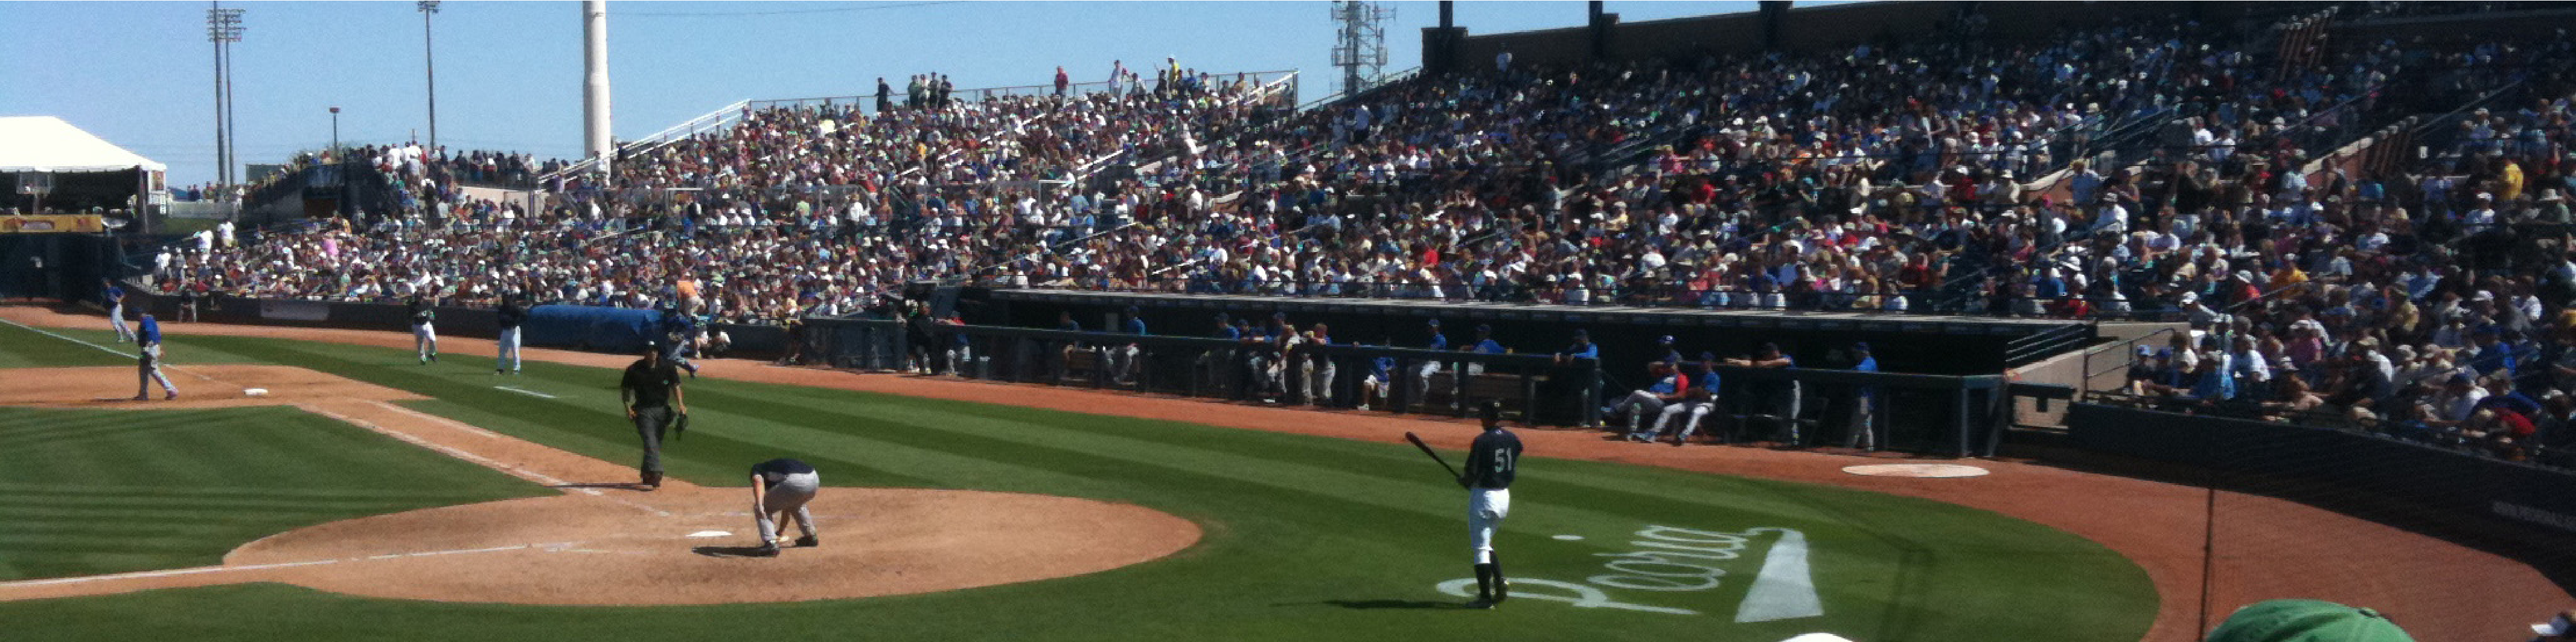
\includegraphics[height=1.5in]{images/sampleteaser}
   \caption{Spring Training 2009, Peoria, AZ.}
 }

\maketitle

\begin{abstract}

In this sample paper, we describe the formatting requirements for
content for the STAR assignment for the Introduction to Computer Graphics class, Fall 2015. Please fill this section with the abstract. This template is based on the SIGGRAPH proceedings template and the following sections will contain dummy sections and text which you can edit.
Use \url{www.overleaf.com} to collaborate and keep track of your document.

\end{abstract}

\begin{CRcatlist}
  \CRcat{I.3.3}{Computer Graphics}{STAR Topic}{CRcat index}
  \CRcat{I.3.7}{Computer Graphics}{STAR Topic}{CRcat index};
\end{CRcatlist}

\keywordlist

%% Required for all content. 

%\copyrightspace

\section{Introduction}

Introduction to your work and the motivation for the STAR topic research. The crucial problem and its solution. The current work will be a survey of the state of the art.
\begin{figure}[h]
	\centering
	\includegraphics[width=3.0in]{images/ferrari_laferrari}
	\caption{This is how you insert an image'}
	\label{fig:ferrari}
\end{figure}


\section{Related Work and Background}

Please fill in this section with the already done work and and summarize the research that has been done, which you will expand upon in the latter sections.

The SIGGRAPH citation format is the ``author year''
format~\cite{Pellacini:2005:LAH}. The year is separated from the
author by a single space~\cite{yee:2000:ssa}. Two authors are
separated by the word ``and''~\cite{parke:1996:CFA}. More than two
authors are represented by the primary author and ``et al.''~\cite{levoy:2000:TDM}.

Multiple citations at a single point in the content are separated by
semicolons~\cite{levoy:2000:TDM,sako:2001:SSB}.


\section{State of the Art}

This will actually have the sections that describe and organize the state of the art research.
Divide the works into subsections and go through them in detail.

Following are the general guidelines for SIGGRAPH submissions:
Please use a serif (Times, Times New Roman, etc.) typeface for the
body of your content. This serif typeface should be used for
everything except the title of your content and section headings,
which should be set in a sans-serif (Helvetica, etc.) typeface.

Your content should be prepared with 9-point text and 10-point line
spacing. This includes the references section. Do not reduce the
typeface size or the line spacing of any part of your content, in an
effort to fit more into a specific number of pages. 

All typefaces used in your content must be embedded in the PDF you
create. 

Paragraphs are prepared without any indentation on the first line, and
with a 10-point-tall space between paragraphs.

Please do not add page numbers to your content. They will be added
during production.






\subsection{\LaTeX}

The ``acmsiggraph'' \LaTeX{} class will faithfully implement the formatting specifications found in this document. Please look at the ``template.tex'' file that accompanies the \LaTeX\ and \BibTeX\ class files, noting these points:
\begin{itemize}
\item In order to leave the correct amount of space clear for the rights management text, you must do two things: 
\begin{enumerate}
\item Use the proper parameter to the \cs{documentclass} command at the top of your source file: use ``tog'' for technical papers accepted to our annual events and published as TOG articles, and use ``conference'' for all other types of content. The parameter determines the amount of space left clear for the rights management text.
\item Use the \cs{copyrightspace} command. It should be placed immediately before the first section of your paper.
\end{enumerate}
If you do not use any parameter to the \cs{documentclass} command, and use the \cs{copyrightspace} command, you'll end up with much more blank space than you want or need.

\item Many authors like to have a large image - called a ``teaser'' image - after the title, author, and affiliation and before the body of the paper. There is a command - \cs{teaser} - which can be used to place such an image. (As has been done in this example document.) Under certain circumstances, the space left clear for the rights management text will move to the base of the right column on the first page. This is acceptable.
\item Use the \cs{keywords} command to define your own keywords, and the \cs{keywordlist} command to prepare and print that block of text.
\item Use the \cs{CRcatlist} environment and the \cs{CRcat} command to define the CR categories appropriate for your paper.
\item There are also ``review'' and ``preprint'' variations of this document class, to be used for material submitted for review, and accepted content to be distributed as a ``preprint.'' These variations have special commands associated with them; see the ``template.tex'' file for more information.
\end{itemize}

\subsection{PDF}

The \LaTeX file can be compiled into a $PDF$

\section{Mathematical Formulae}
The following section can be found at \url{www.sharelatex.com}.
%--------------------------------------------------------------------------------
\subsection{First example}

The well known Pythagorean theorem \(x^2 + y^2 = z^2\) was 
proved to be invalid for other exponents. 
Meaning the next equation has no integer solutions:

\[ x^n + y^n = z^n \]


%--------------------------------------------------------------------------------

\subsection{Second example}

In physics, the mass-energy equivalence is stated by the equation $E=mc^2$, discovered in 1905 by Albert Einstein.

The mass-energy equivalence is described by the famous equation
$$E=mc^2$$
discovered in 1905 by Albert Einstein. 
In natural units ($c$ = 1), the formula expresses the identity
\begin{equation}
E=m
\end{equation}

\subsection{Third example}

This is a simple math expression \(\sqrt{x^2+1}\) inside text. 
And this is also the same: 
\begin{math}
	\sqrt{x^2+1}
\end{math}
but by using another command.

This is a simple math expression without numbering
\[\sqrt{x^2+1}\] 
separated from text.

This is also the same:
\begin{displaymath}
\sqrt{x^2+1}
\end{displaymath}

\ldots and this:
\begin{equation*}
	\sqrt{x^2+1}
\end{equation*}

\subsection{Fourth example}
Multi line expressions
\begin{align}
2x^2 + 3(x-1)(x-2) & = 2x^2 + 3(x^2-3x+2)\\ \nonumber &= 2x^2 + 3x^2 - 9x + 6\\ &= 5x^2 - 9x + 6
\end{align}

\subsection{Advanced examples}
Refer to \url{https://en.wikibooks.org/wiki/LaTeX/Advanced\_Mathematics} for more advanced examples.

\[
\lim_{x\to 0}{\frac{e^x-1}{2x}}
\overset{\left[\frac{0}{0}\right]}{\underset{\mathrm{H}}{=}}
\lim_{x\to 0}{\frac{e^x}{2}}={\frac{1}{2}}
\]

\begin{equation}
x = a_0 + \frac{1}{\displaystyle a_1 
	+ \frac{1}{\displaystyle a_2 
		+ \frac{1}{\displaystyle a_3 + a_4}}}
\end{equation}

\section{Macros}
The following section can be found at \url{www.sharelatex.com}.
The commands have been defined as macros before the beginning of the document. Scroll up to check them.
%\newcommand{\R}{\mathbb{R}}
%\newcommand{\bb}[1]{\mathbb{#1}}
%\newcommand{\plusbinomial}[3][2]{(#2 + #3)^#1}


%-----------------------------------------------------------------------------------
%Example, simple usage of commands and environments
In a document there are different types of \textbf{commands} that define the way the
elements are displayed. This command may insert special elements: $\alpha \beta \Gamma$
%-----------------------------------------------------------------------------------
%-----------------------------------------------------------------------------------
%Commands with extra parameters
Example a list
\begin{itemize}
	\item First item
	\item[\S] Second item
\end{itemize}
%-----------------------------------------------------------------------------------
%-----------------------------------------------------------------------------------
%Example using a simple user-defined command
The set of real numbers are usually represented by a blackboard bold capital r: \( \R \). 
%-----------------------------------------------------------------------------------

%giving vertical space
\vspace{1cm}

%-----------------------------------------------------------------------------------
%Example using a simple user-defined command
Other numerical systems have similar notations. The complex numbers \( \bb{C} \), the rational numbers \( \bb{Q} \) and the integer numbers \( \bb{Z} \).
%-----------------------------------------------------------------------------------

%-----------------------------------------------------------------------------------
%Example using a simple user-defined command with optional parameters
To save some time when writing too many expressions with exponents is by defining a new command to make simpler:

\[ \plusbinomial{x}{y} \]

And even the exponent can be changed

\[ \plusbinomial[4]{y}{y} \]
%-----------------------------------------------------------------------------------
%-----------------------------------------------------------------------------------
%Example, renameing and existing command
%Command to redefine \S
\renewcommand{\S}{\mathbb{S}}

The riemann sphere (the complex numbers plus $\infty$) is sometimes represented by \( \S \)
%-----------------------------------------------------------------------------------


\section{Tables}

A simple table can be constructed using \LaTeX

\begin{center}
	\begin{tabular}{||c c c c||} 
		\hline
		Col1 & Col2 & Col2 & Col3 \\ [0.5ex] 
		\hline\hline
		1 & 6 & 87837 & 787 \\ 
		\hline
		2 & 7 & 78 & 5415 \\
		\hline
		3 & 545 & 778 & 7507 \\
		\hline
		4 & 545 & 18744 & 7560 \\
		\hline
		5 & 88 & 788 & 6344 \\ [1ex] 
		\hline
	\end{tabular}
\end{center}

For more complicated formatting refer to \url{https://www.sharelatex.com/learn/Tables}

Before the start of the document you need certain settings.
%\usepackage[table]{xcolor}
%
%\setlength{\arrayrulewidth}{1mm}
%\setlength{\tabcolsep}{18pt}
%\renewcommand{\arraystretch}{2.5}

\newcolumntype{s}{>{\columncolor[HTML]{AAACED}} p{0.15\textwidth}}

\arrayrulecolor[HTML]{DB5800}
\begin{table}[h]
\begin{tabular}{ |s|p{0.05\textwidth}|p{0.05\textwidth}|  }
	\hline
	\rowcolor{lightgray} \multicolumn{3}{|c|}{Country List} \\
	\hline
	Country Name    or Area Name& ISO ALPHA 2 Code &ISO ALPHA 3 \\
	\hline
	Afghanistan & AF &AFG \\
	\rowcolor{gray}
	Aland Islands & AX & ALA \\
	Albania   &AL & ALB \\
	Algeria  &DZ & DZA \\
	American Samoa & AS & ASM \\
	Andorra & AD & \cellcolor[HTML]{AA0044} AND    \\
	Angola & AO & AGO \\
	\hline
\end{tabular}
\end{table}

\section{Images}
The following code arranges 2 images and a table
\begin{figure*}
\centering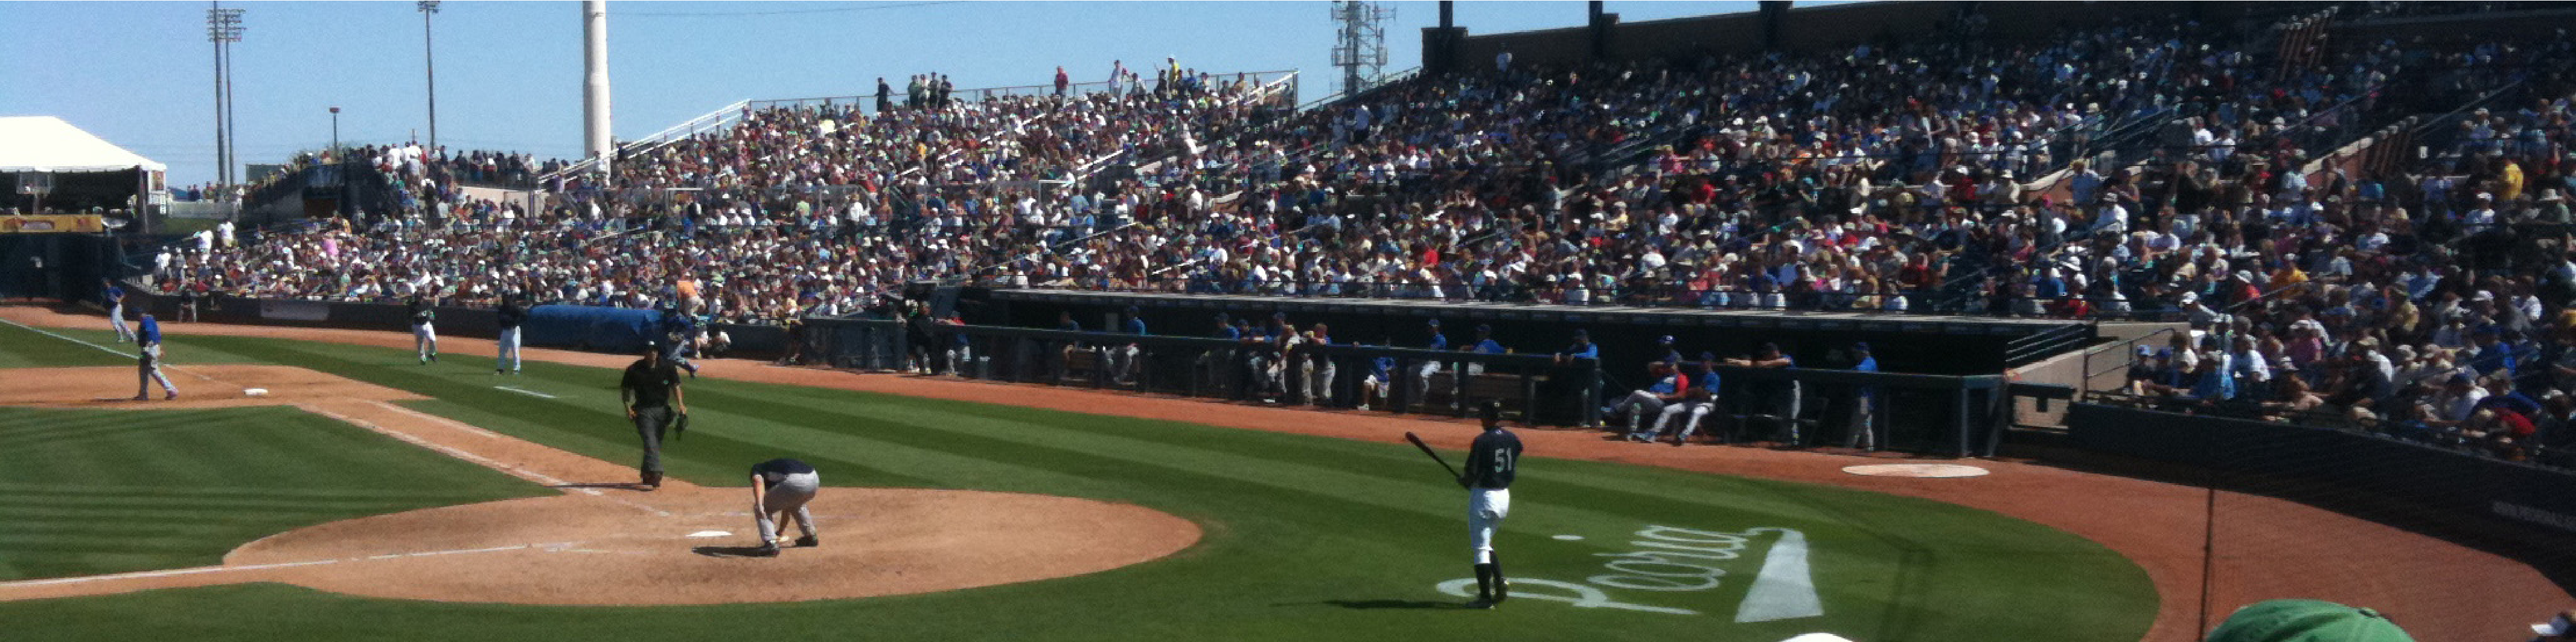
\includegraphics[width=.9\linewidth,height=2in]{images/sampleteaser}\par
\caption{This is a figure caption}

\vspace*{\floatsep}

\begin{minipage}{.5\linewidth}
\centering
\begin{tabular}{ccc}
\hline
One & Two & Three \\
Three & One & Two \\
Two & Three & One \\
\hline
\end{tabular}
\captionof{table}{This is a table caption}
\end{minipage}%
\begin{minipage}{.5\linewidth}
\centering\includegraphics[width=.8\linewidth]{images/ferrari_laferrari}
\captionof{figure}{This is a figure caption}
\end{minipage}
\end{figure*}

\section{Contact Information}

If you have questions or suggestions regarding this document, please
contact Stephen Spencer at ``spencer@cs.washington.edu''.

\section*{Acknowledgements}

To Robert, for all the bagels.

\bibliographystyle{acmsiggraph}
\nocite{*}
\bibliography{template}
\end{document}